\documentclass{article}
\usepackage{pgfplots}
\usepackage{siunitx}
\usepackage[paperheight=2.9in,paperwidth=3.9in,margin=0in]{geometry}
\pgfplotsset{compat=1.17}
\usepgfplotslibrary{external}
\usepgfplotslibrary{fillbetween}

\tikzexternalize

\definecolor{pastelred}{rgb}{1.0, 0.41, 0.38}
\definecolor{pastelmagenta}{rgb}{0.96, 0.6, 0.76}\definecolor{pastelpink}{rgb}{1.0, 0.82, 0.86}

\begin{document}
 \pagenumbering{gobble} 
\pgfplotsset{every axis plot/.append style={line width=1pt, font=\large,}}
\tikzsetnextfilename{test.pdf}

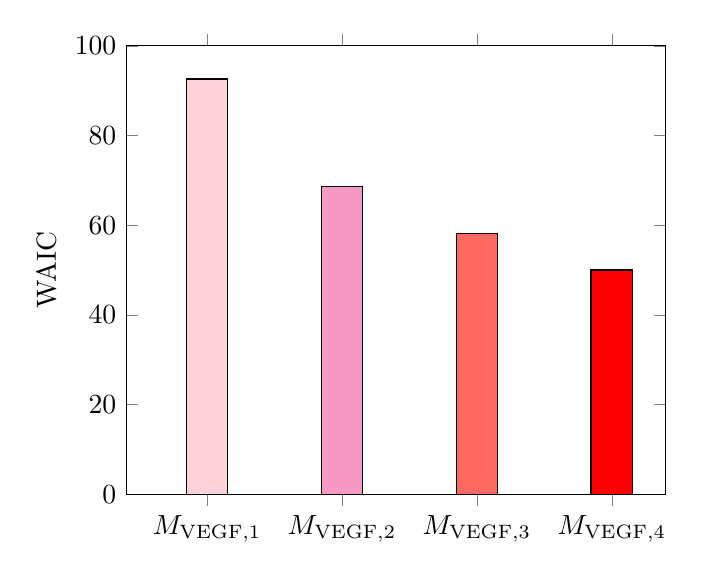
\begin{tikzpicture}
    \begin{axis}[
        ybar,
        bar shift=0pt,
        bar width=15pt,
        ylabel = {WAIC},
        xmin=0.7,
        xmax=2.7,
        xtick={1,1.5,2,2.5},
        xticklabels={$M_{\text{VEGF},1}$,$M_{\text{VEGF},2}$,$M_{\text{VEGF},3}$,$M_{\text{VEGF},4}$},
        scaled y ticks = false,
        ymin=0, ymax=100,
    ]
        \addplot[style={black,fill=pastelpink,mark=none}] coordinates {(1,23+19.5+50.1)};
        \addplot[style={black,fill=pastelmagenta,mark=none}] coordinates {(1.5,11+19.5+38.1)};
        \addplot[style={black,fill=pastelred,mark=none}] coordinates {(2,12+16.1+30)};
        \addplot[style={black,fill=red,mark=none}] coordinates {(2.5,10+19.7+20.3)};
    \end{axis}
\end{tikzpicture}
\end{document}

